\chapter{Methods and Procedures} \label{ch:methods}

In this section, the methods for extracting homology information, \ie~Betti numbers, from images generated by simulating the Gray-Scott system are outlined. \refsect{sect:thresholding} describes the process of preparing the images for computation and the considerations and problems that arise. In \refsect{sect:entropy}, the Betti numbers are used to calculate the entropy of the Gray-Scott system as parameters are varied. For information on how the pattern images were generated in the first place, see \refsect{ch1:gs-simulation}.

\section{Obtaining Betti numbers}

Given the complicated overview of cubical homology theory given in \refsect{ch2:cubicalhomology}, one might expect extracting the Betti numbers from an image to be a difficult undertaking. Fortunately, \textsc{CHomP}, (Computational Homology Project), a homology software package developed by the group of Konstantin Mischaikow (Mathematics '79) at Rutgers University (formerly at Georgia Tech), facilitates this process\rf{chomp}. Furthermore, the way it works is extremely intuitive, essentially counting clusters of adjacent pixels. \textsc{CHomP} requires a 2-bit binary image as input.\footnote{That is, an image with \emph{only} black and white pixels.} Since the images output by the Gray-Scott simulation are greyscale (see \refsect{ch1:gs-simulation}), they must first be converted to a 2-bit image.

\subsection{Thresholding} \label{sect:thresholding}

The output of the Gray-Scott simulation is a series of 8-bit greyscale images, \ie~there are 256 possible shades of grey (0 is black, 255 is white). The color map is such that concentrations $V_{min} = 0.0 \rightarrow 255$ and $V_{max} = 0.4 \rightarrow 0$. In other words, white and black indicate low and high concentration of $V$ respectively.\footnote{$V_{max}$ was chosen based on the average maximum of $V \approx 0.4$ for all the patterns examined.} Each image is then thresholded at some value $T \in [0,255]$. That is, all pixels with intensity $< T$ are now black and those with intensity $> T$ are now white.

\begin{figure}[p]
	\centering
	\begin{subfigure}[b]{0.25\textwidth}
                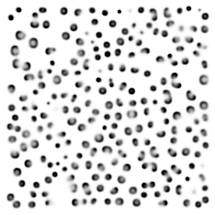
\includegraphics[width=\textwidth]{alpha_v_grey.png}
                \caption{$\alpha$ in greyscale.}
                \label{fig:alpha_grey}
        \end{subfigure} \quad
	\begin{subfigure}[b]{0.25\textwidth}
                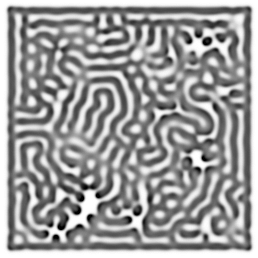
\includegraphics[width=\textwidth]{gamma_v_grey.png}
                \caption{$\gamma$ in greyscale.}
                \label{fig:gamma_grey}
        \end{subfigure}\quad
	\begin{subfigure}[b]{0.25\textwidth}
                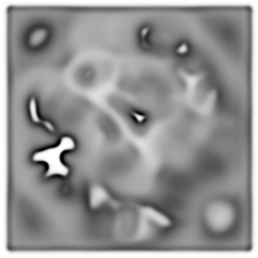
\includegraphics[width=\textwidth]{beta_v_grey.png}
                \caption{$\beta$ in greyscale.}
                \label{fig:beta_grey}
        \end{subfigure}\hfill \\
        ~ %add desired spacing between images, e. g. ~, \quad, \qquad, \hfill etc.
          %(or a blank line to force the subfigure onto a new line)
	\begin{subfigure}[b]{0.25\textwidth}
                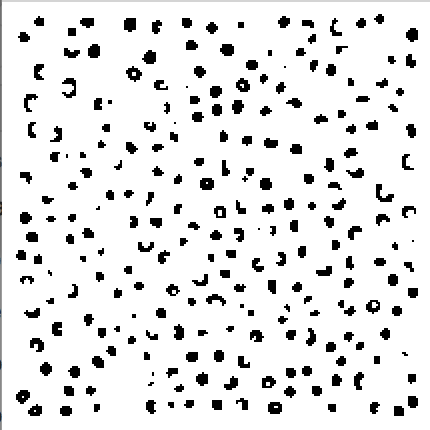
\includegraphics[width=\textwidth]{alpha_v_thresh112.png}
                \caption{$\alpha$, $T =$ 112.}
                \label{fig:alpha_112}
        \end{subfigure} \quad
	\begin{subfigure}[b]{0.25\textwidth}
                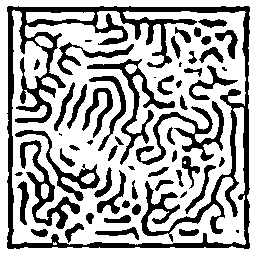
\includegraphics[width=\textwidth]{gamma_thresh112.png}
                \caption{$\gamma$, $T =$ 112.}
                \label{fig:gamma_112}
        \end{subfigure}\quad
        \begin{subfigure}[b]{0.25\textwidth}
                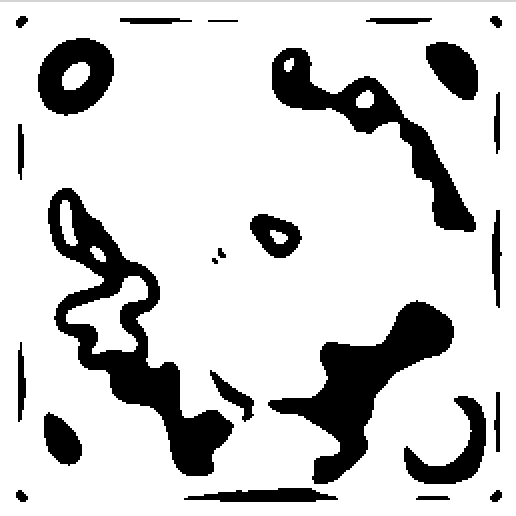
\includegraphics[width=\textwidth]{beta_v_thresh112.png}
                \caption{$\beta$, $T =$ 112.}
                \label{fig:beta_112}
        \end{subfigure} \hfill \\
        
        \begin{subfigure}[b]{0.25\textwidth}
                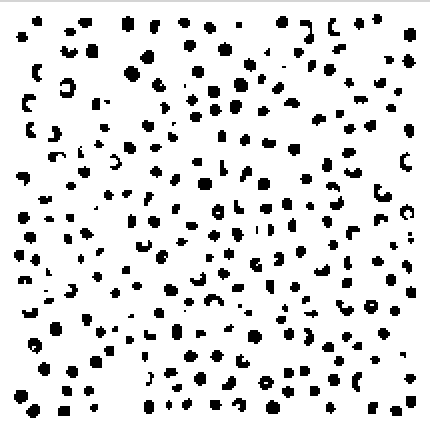
\includegraphics[width=\textwidth]{alpha_v_thresh128.png}
                \caption{$\alpha$, $T =$ 128.}
                \label{fig:alpha_128}
        \end{subfigure} \quad
         \begin{subfigure}[b]{0.25\textwidth}
                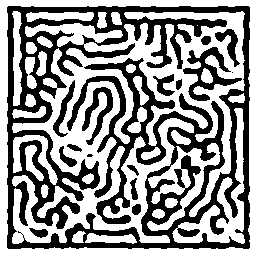
\includegraphics[width=\textwidth]{gamma_thresh128.png}
                \caption{$\gamma$, $T =$ 128.}
                \label{fig:gamma_128}
        \end{subfigure}\quad
        \begin{subfigure}[b]{0.25\textwidth}
                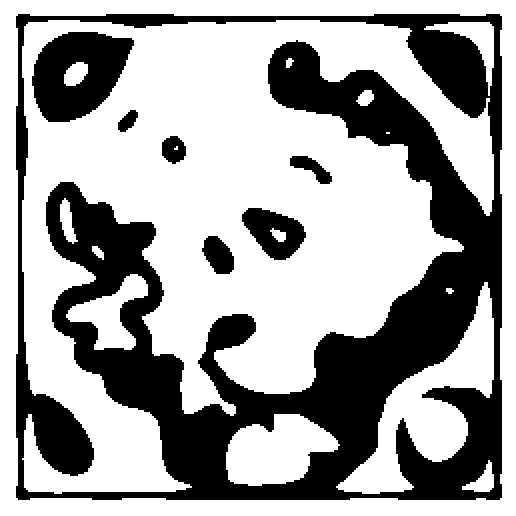
\includegraphics[width=\textwidth]{beta_v_thresh128.png}
                \caption{$\beta$, $T =$ 128.}
                \label{fig:beta_144}
        \end{subfigure} \hfill \\
        
        \begin{subfigure}[b]{0.25\textwidth}
                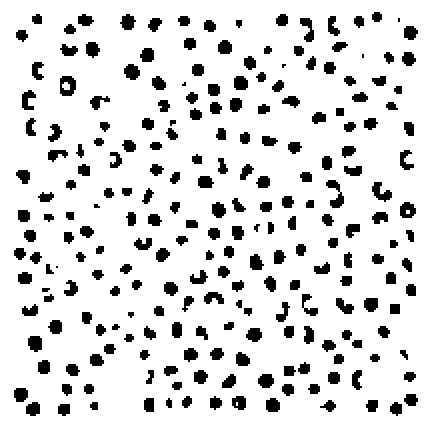
\includegraphics[width=\textwidth]{alpha_v_thresh144.png}
                \caption{$\alpha$, $T =$ 144.}
                \label{fig:alpha_144}
        \end{subfigure} \quad
         \begin{subfigure}[b]{0.25\textwidth}
                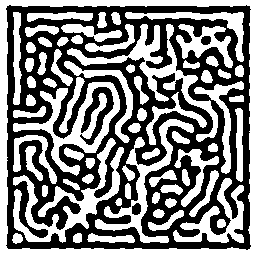
\includegraphics[width=\textwidth]{gamma_thresh144.png}
                \caption{$\gamma$, $T =$ 144.}
                \label{fig:gamma_144}
        \end{subfigure} \quad
         \begin{subfigure}[b]{0.25\textwidth}
                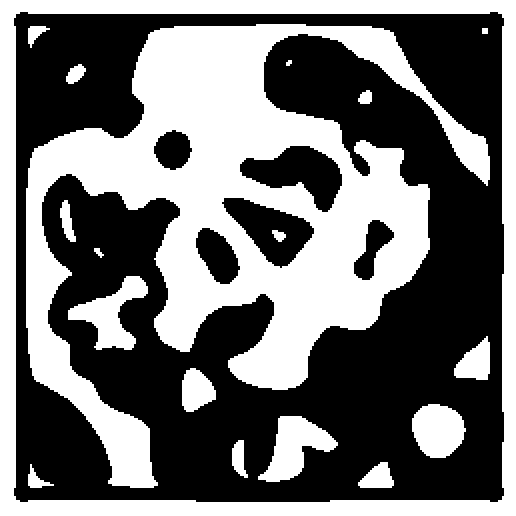
\includegraphics[width=\textwidth]{beta_v_thresh144.png}
                \caption{$\beta$, $T =$ 144.}
                \label{fig:beta_144}
        \end{subfigure} \hfill
        \caption{Patterns $\alpha$, $\gamma$, and $\beta$ at various thresholds. Some features of less stable patterns such as $\gamma$ and $\beta$ are lost when thresholded. Thresholds slightly higher than 128 tend to capture the features of the original pattern better.} \label{fig:thresholds}
\end{figure}

A logical choice for $T$ is the median pixel intensity of the image\rf{krishan_2007}. But, in the case of sparse patterns like $\alpha$ and $\epsilon$ (\refFigs{fig:alpha_sample}{fig:epsilon_sample} respectively), this results in a completely black image since the median is very high. Although other adaptive methods of thresholding exist\rf{mischaikow_2002}, the definitive answer to thresholding problems is \emph{persistent homology}, a more sophisticated computational homology technique which is a large leap in terms of complexity and outside the scope of this thesis\rf{persistence_2008}. This approach is concerned with the ``birth'' and ``death'' of homology components as the threshold is varied in a away that circumvents the need for a threshold altogether. Persistent homology has recently seen great success in analyzing large sets of nonlinear data\rf{weinberger_2011}.

Short of persistent homology, another reasonable choice would be to split right down the middle, $T = 128$, but as \refFigs{fig:thresholds}{fig:bplots_gamma} illustrate, some information can be lost in the process. Thus the optimal choice of threshold depends entirely on the characteristics of the image. The patterns produced by the Gray-Scott system are varied and no single value of $T$ is ideal for all $(F, k)$, but emperically, $T$ that is near 128 better agrees with the characteristics of the original pattern. After experimentation, the value $T = 144$ was chosen to perform all the calculations for Gray-Scott patterns of chemical $V$.

Provided in the \textsc{CHomP} software package is a method for simply thresholding images, \texttt{chomp-greyscale-to-cubical} (which takes a single image input, a threshold value, and an output filename). The output is a text file which contains the coordinates of white pixels.

\begin{sidewaysfigure}[p]
	\centering
	\begin{subfigure}[b]{0.45\textwidth}
                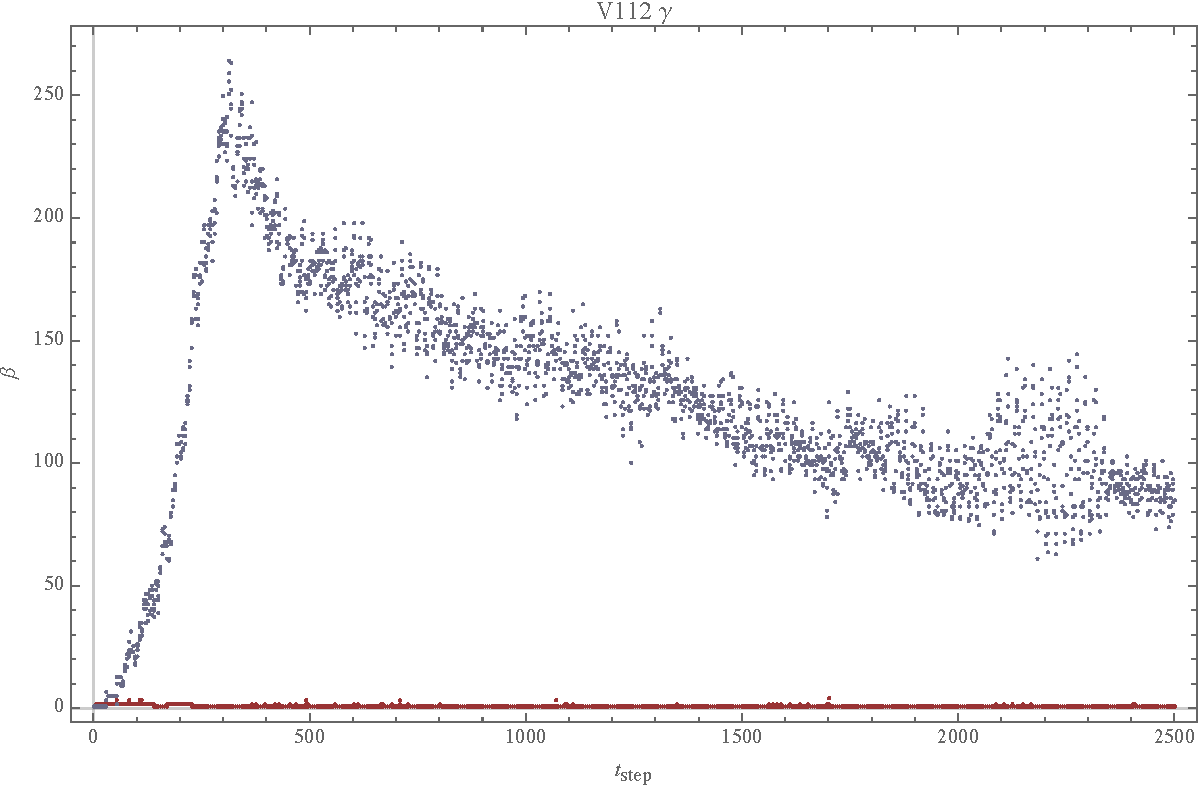
\includegraphics[width=\textwidth]{bplot_gamma112}
                \caption{$\gamma$, $T = 112$.}
                \label{fig:bplot_gamma112}
        \end{subfigure} \quad
	\begin{subfigure}[b]{0.45\textwidth}
                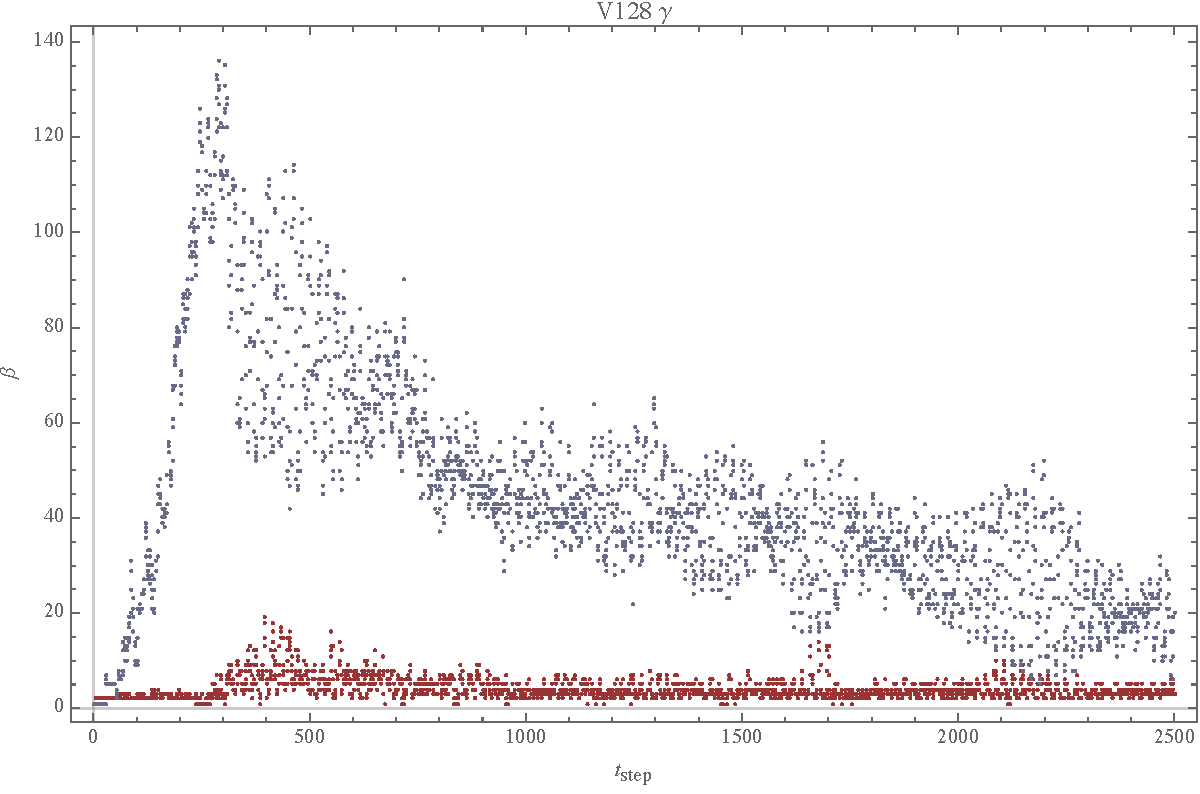
\includegraphics[width=\textwidth]{bplot_gamma128}
                \caption{$\gamma$, $T = 128$.}
                \label{fig:bplot_gamma128}
        \end{subfigure} \hfill \\
        %
	\begin{subfigure}[b]{0.45\textwidth}
                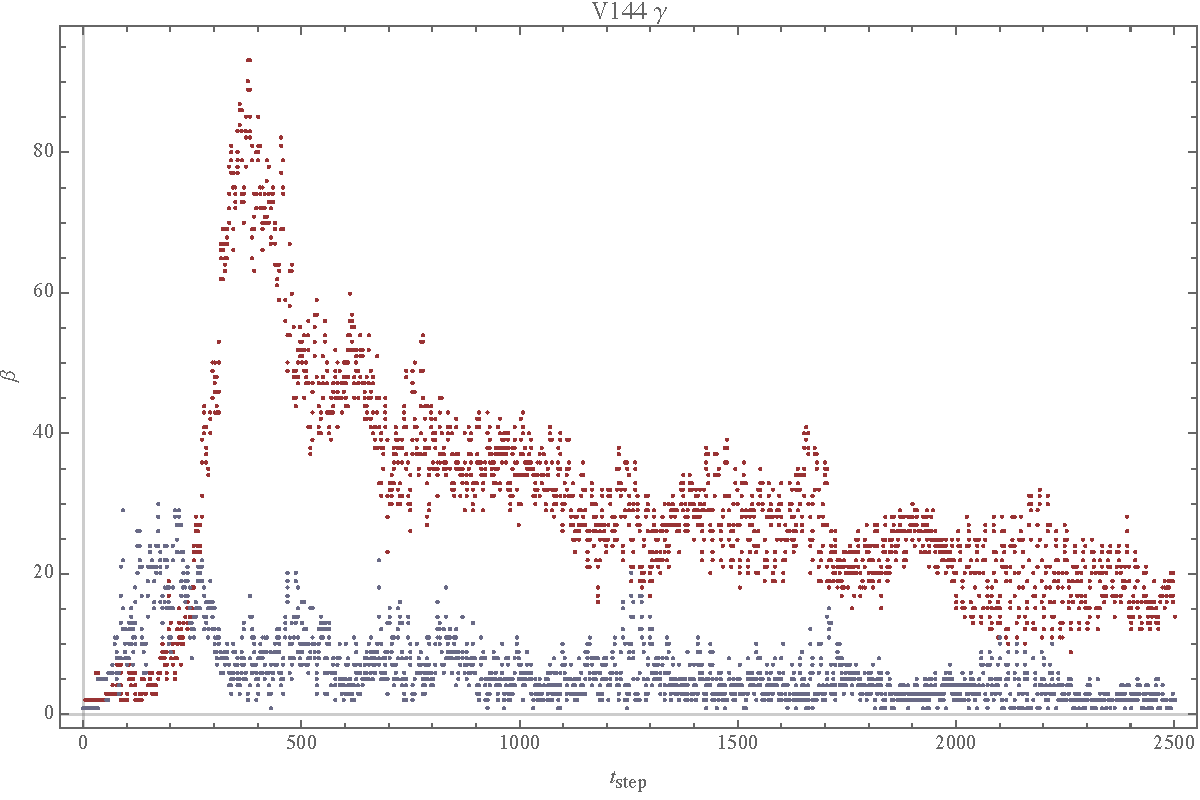
\includegraphics[width=\textwidth]{bplot_gamma144}
                \caption{$\gamma$, $T = 144$.}
                \label{fig:bplot_gamma144}
       \end{subfigure} \quad
       \begin{subfigure}[b]{0.45\textwidth}
                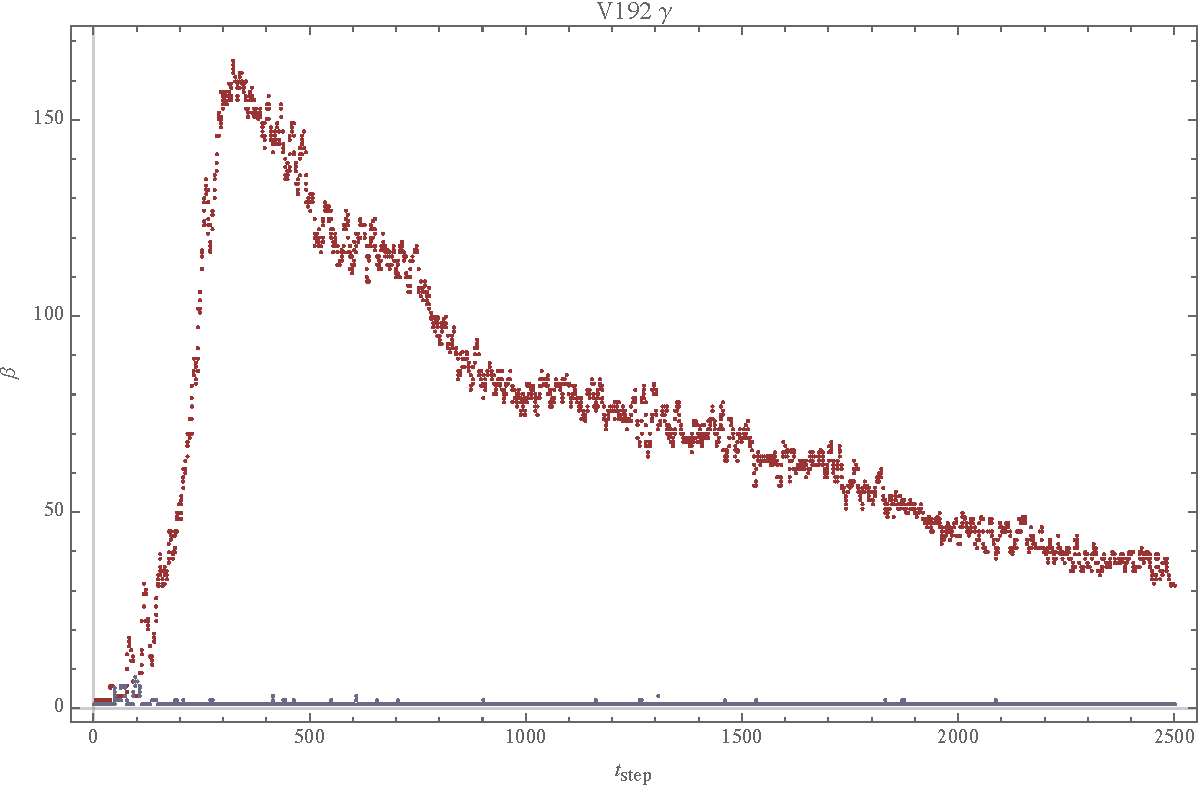
\includegraphics[width=\textwidth]{bplot_gamma192}
                \caption{$\gamma$, $T = 192$.}
                \label{fig:bplot_gamma192}
        \end{subfigure}
        
        \caption{A plot of the time series of Betti numbers for pattern $\gamma$. The zeroth Betti number $\beta_0$ is shown in red and the first Betti number $\beta_1$ shown in blue. Different thresholds $T =$ 112, 128, 144, and 192 demonstrate the dramatic effect of thresholding on the calculation of Betti numbers for some patterns. For very high and low $T$, the image loses any resemblance to the original image (since it will appear mostly black or white). Slightly varying the threshold near 128, however, can help minimize the loss of information and remain truer to the original image. Interactive charts for each pattern type are available online at \url{http://joelhawkins.info/thesis}.} \label{fig:bplots_gamma}
\end{sidewaysfigure}

\newpage
\subsection{Computational homology} \label{sect:chomping}

Once the images are thresholded at some value, the \textsc{CHomP} method \texttt{chomp-cubical} processes and returns Betti numbers $\beta_0$, $\beta_1$, and $\beta_2$.  A single calculation of Betti numbers takes about 1-3s on a 4.2 GHz Intel i7 processor constituting the greatest bottleneck in the process. \refFig{fig:spiral_thresh} shows the intermediate stages of calculating Betti numbers for a single choice of $F,k$ values. This process is performed for each of 2,500 text files produced by thresholding to generate a single CSV file of the Betti numbers $\beta_0$, $\beta_1$, and $\beta_2$ for each time step.\footnote{The Betti number $\beta_2$ is included only for posterity; $\beta_2$ = 0 for all time steps since the images are only 2D.}

\begin{figure}[h]
	\centering
	\begin{subfigure}[b]{0.33\textwidth}
                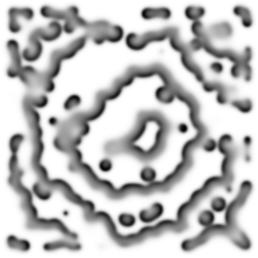
\includegraphics[width=\textwidth]{spiral_b0-5_b1-32.png}
                \caption{}
                \label{fig:spiral_grey}
        \end{subfigure} \quad
	\begin{subfigure}[b]{0.33\textwidth}
                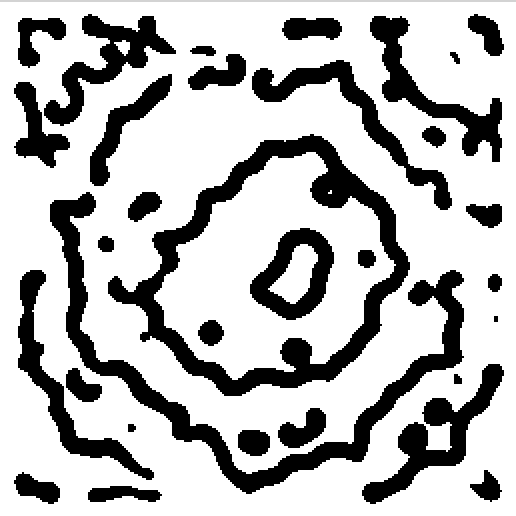
\includegraphics[width=\textwidth]{spiral_144.png}
                \caption{}
                \label{fig:spiral_144}
        \end{subfigure}
        \caption{On the left is a spiral pattern with $(F, k) = (0.035, 0.060)$ while the figure on the right shows the pattern thresholded at $T = 144$. The Betti numbers for this pattern, as calculated by \textsc{CHomP}, are $\beta_0 = 32$, $\beta_1 = 5$.}
        \label{fig:spiral_thresh}
\end{figure}

\section{Calculating entropy} \label{sect:entropy}

In physics, entropy usually denotes the amount of ``disorder'' of a system. Shannon's entropy, $S(X)$, indicates the average amount of information that an observer gains \emph{after} measuring a realized outcome $x$ of the random variable $X$\rf{grunwald_2004}. We wish to use homology information to provide a sense of how predictable (how complex) the dynamics of the Gray-Scott system are for a given choice of parameters ($F$ and $k$). In general, the Shannon entropy $S$ of some variable $X$ with possible values $\{ x_1, \ldots, x_N \}$ and probability distribution $P(x_i) = P_i$ is defined by
\begin{align} \label{eq:shannon}
	S(X) = - \sum_{i=1}^{N} P_i \log{ P_i}.
\end{align}
In our case, the Shannon entropy gives a picture of the average minimum number of topological ``states'' required to describe the system based on the frequency of the states explored by the system (\ie how often some state occurs in the time series).\footnote{The units of $S$ are called ``nats'' when the $\log$ in \refeq{eq:shannon} is the natural logarithm.} A \emph{state} in this case is taken to be a unique pair of Betti numbers $s_i = \{ \beta_0, \beta_1 \}_i$ at the $i$th time step. Although $s_i$ in general doesn't describe a \emph{unique} pattern (any two states such that $s_i = s_j$ could look very different), it captures the fundamental topology of the system at that moment. Furthermore, the set of states within a given set of parameters (any $F, k$) is more meaningful. For example, if we observe the topology of state $s_i$ for pattern $\alpha$, then we can make an informed prediction as to what some other state $s_j$ might look like for that pattern (assuming we know what the characteristic/steady-state pattern for $\alpha$ looks like). In general, we would expect higher entropy for more dynamic, complex patterns.

\begin{figure}[h]
	\centering
	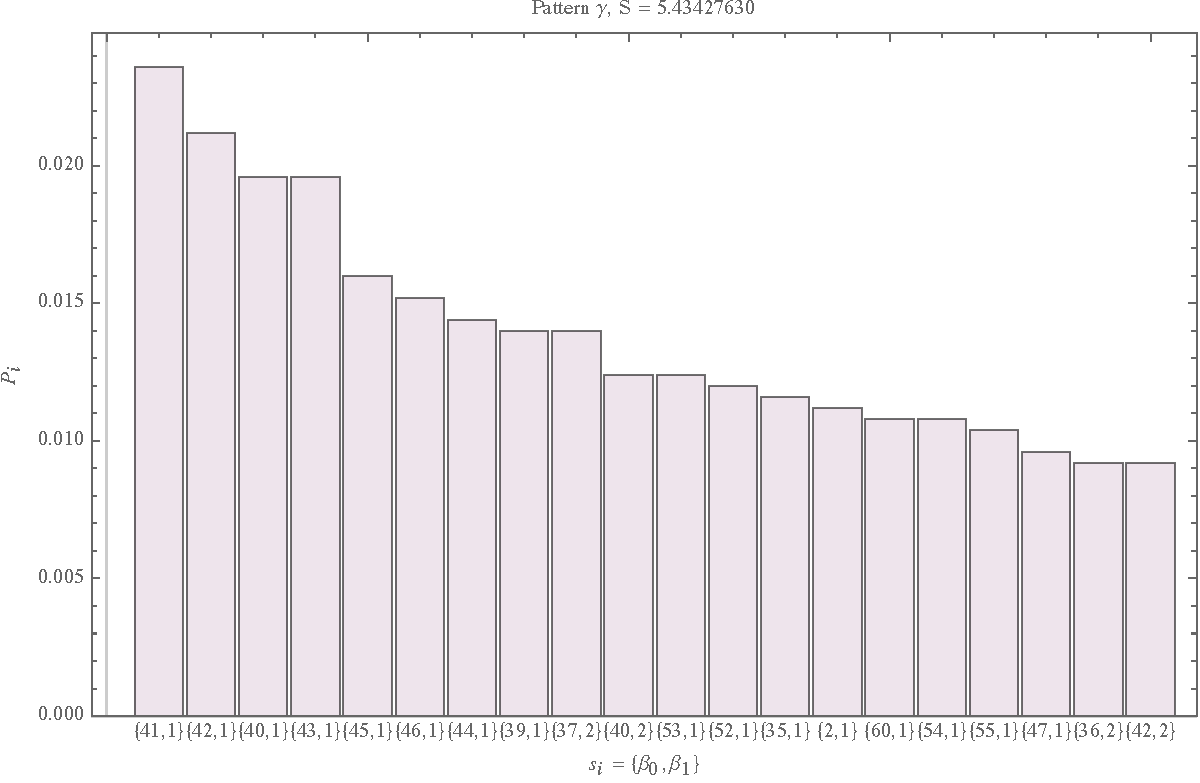
\includegraphics[width=\textwidth]{gamma_phist}
                \caption{The probability $P_i$ of the 20 most probable states $s_i$ for pattern $\gamma$ with $(F, k) = (0.022,\, 0.051)$. The entropy of this system is $S = 5.43427630$ nats. Interactive charts for each pattern type are available online at \url{http://joelhawkins.info/thesis}.}
                \label{fig:gamma_phist}
\end{figure}

For $N$ total (non-unique) states equal to the number of time steps, the probability $P_i$ of state $s_i$ given $N_i$, the number of times state $s_i$ occurs, is simply
\begin{align} \label{eq:Pi}
	P_i = \frac{N_i}{N}.
\end{align}
\refFig{fig:gamma_phist} charts the twenty states, $s_i$, with the highest probability, $P_i$ (\ie the twenty most probable states) for the pattern $\gamma$ (\refFigs{fig:gamma_sample}{fig:gamma_grey}). More dynamic patterns have a more even distribution of many states, each with lower $P_i$. Patterns like $\mu$ (\refFig{fig:mu_sample}) that evolve slowly have a very small number of possible states each with high $P_i$ and therefore a very low entropy.

Since we can use homology information, namely the time series of Betti numbers, to calculate the entropy of a single pattern, we might ask if we can use this information to gain insight into the dynamics of the entire Gray-Scott pattern-forming system. In the following chapter, we examine how the entropy changes as parameters are varied, how it compares to Pearson's analysis, and investigate other information that can be derived from the time series of Betti numbers.


